%Short description of the posible actions in feedjam
FeedJam is a Twitter application that uses the Twitter REST API to retrieve data from Twitter. When entering the page the user can use the search field to search for their interests. The trending topics of the last 24 hours is also presented on the front page. Once the users has entered a search term the API's search method to retrieve tweets based on a query term. 
The system responds with relevant tweets from the last two weeks. It also retrieves information about the user that wrote the tweet. The application stores tweets, user information and trending topics in a database. 

%Sections
\subsection{Structure}
\subsubsection{MVC} %torstein view delen, lisa model og contoller

\subsubsection{The View}
The view is the component of MVC-applications which receives input from the user and displays output from the controllers and model. While the model and the controllers contain logic in order to do database interactions and data manipulation the view in general only contains logic in the form of simple if-statements and loops in order to display the content assigned by the controller. The view is also the component which, in web applications, contains the HTML markup, CSS-styling and javascript needed to provide users with the intentioned graphical design and user experience.

Within the context of Spring views are written in a language called JSP. JSP, Java Server Pages, is an alternative form of Java intended to be used within HTML and then compiled server side. While it is possible to write entire applications in JSP it is generally not considered good practice to do any logic outside logic specifically needed in order to display content from within the objects assigned to the view.

%hva MVC er
%hvor ting er
\subsubsection{Interaction between view and controller} %snorre

\subsubsection{Interaction between controller and model} %lisa
%information flow, hvordan ting skjer
%brukt desingn patterns 
{\bf packages}
\begin{itemize}
  \item uib.info323.twitterAWSM contains the controllers
  \item uib.info323.twitterAWSM.exceptions contains exceptions
  \item uib.info323.twitterAWSM.io contains interfaces for interacting with persistence layer (postfixed -DAO), interfaces for searching the Twitter API (postfixed -SearchFactory) and interfaces for crating model object (postfixed -Factory).
  \item uib.info323.twitterAWSM.io.impl contains MySql implementations, Json implementations and model implementations. 
  \item uib.info323.twitterAWSM.io.rowmapper contains rowmappers used in accessing persistence layer
  \item uib.info323.twitterAWSM.model.impl contains model implementations
  \item uib.info323.twitterAWSM.model.interfaces contains model interfaces
  \item uib.info323.twitterAWSM.model.impl contains model implementations
  \item uib.info323.twitterAWSM.pagerank contains PageRank/UserRank implementation
  \item uib.info323.twitterAWSM.model.utils contains parsers etc.
\end{itemize}


\subsection{Layout} %torstein
%beskriver layout, hvordan ting ser ut, hvorfor det ser sånn ut.

\subsubsection{Defining the concept}
Since FeedJam is an effort to ease the consumption of tweets and Twitter conversations through the use of Page Rank and tweet ranking we needed a good way of displaying the results of said rankings graphically. Normally search engines are able to sort the output of searches after relevance due to their non-restricted access to their own database. However, in the case of Twitter we only have access to a severely limited number of tweets through their public API. In addition to this we believe that the shere amount of new tweets every minute would be a too large amount to effectively process for our computers and server even if we were able to fully access the Twitter database. Therefore a normal sorted listing of search results were rendered effectively impossible. Another aspect to take into consideration is the conversational nature of many tweets. It was decided that the FeedJam layout would somehow follow the conversation without sorting tweets but simultaniously helping users skim through large conversations quickly and help users see important tweets.

Normally when browsing through lists of unsorted rated content we are explicitly shown the content's rating. This is true for instance in the case of movie or music listings where a grade is displayed, often in the form of a dice or a number. While we did want to display our rating we also wanted to provide the user with more powerfull visual cues to the generated importance measure of tweets in order to follow our layout goal of easing skimming of large conversations. Hence we decided on the use of purely visual cues in the form of colours or transparency in order to differentiate between rankings.

\subsubsection{Early efforts}
Early concepts placed tweets in a list format. The thinking behind using a simple list format is that Twitter in its current iteration use a similar design to display tweets. This did however prove to be an inefficient use of the available space in the browser, and was quickly scrapped in favour of a grid-based layout.

\begin{figure}[ht]
    \begin{minipage}[b]{0.5\linewidth}
        \centering
        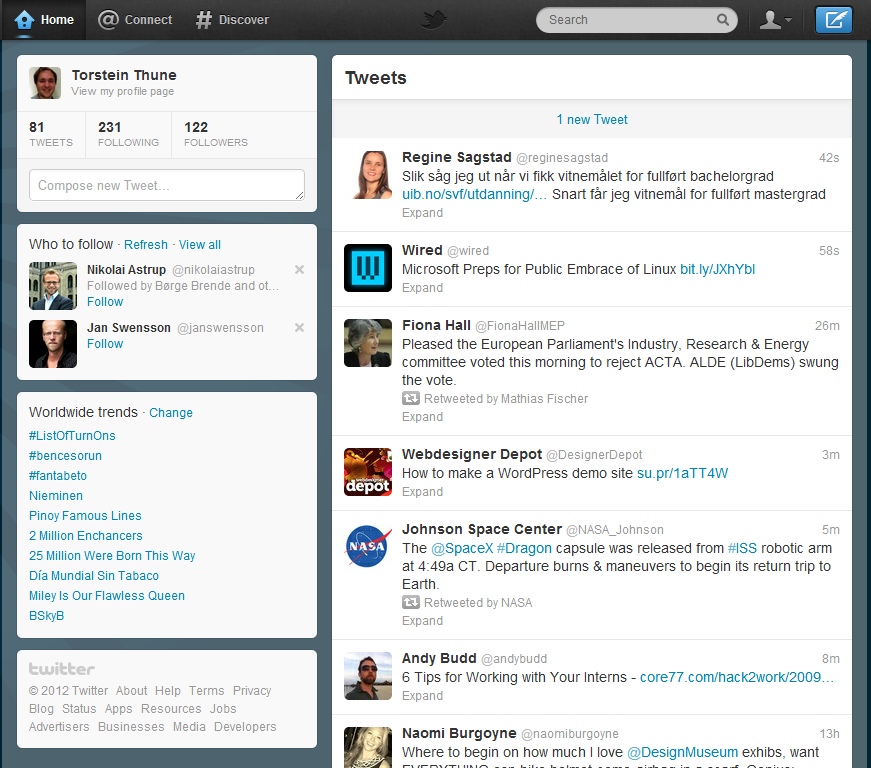
\includegraphics[width=\textwidth]{figures/twitter_list}
        \caption{Twitter in its current iteration.}
        \label{fig:Twitter}
    \end{minipage}
    \hspace{0.5cm}
    \begin{minipage}[b]{0.5\linewidth}
        \centering
        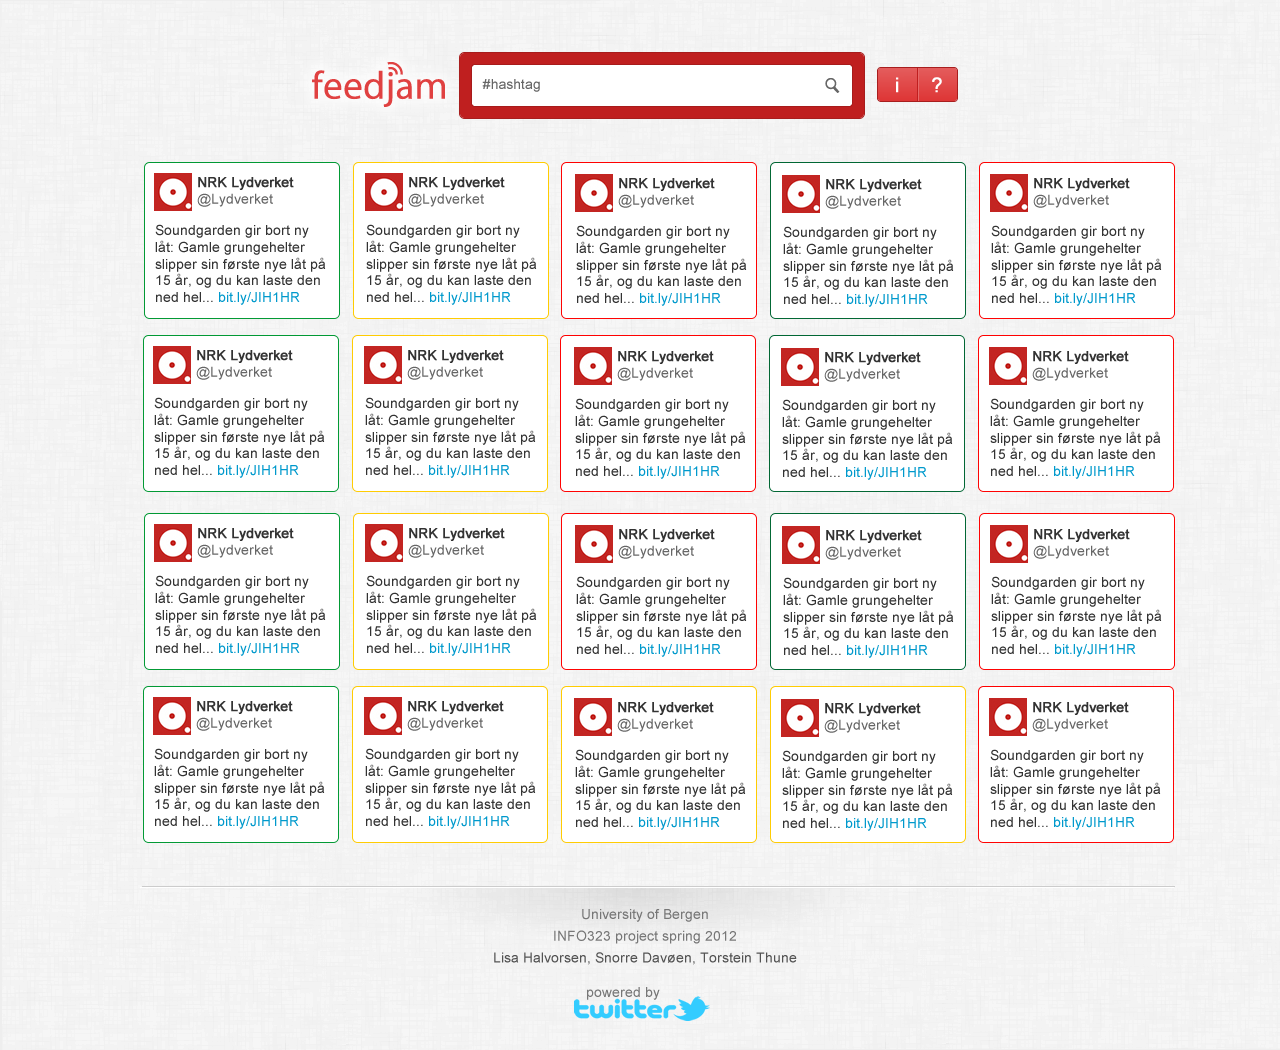
\includegraphics[width=\textwidth]{figures/layout_colour_borders}
        \caption{Early FeedJam concept}
        \label{fig:FeedJamColours}
    \end{minipage}
\end{figure}

We did also experiment with using colours to display the importance of tweets. Early thoughts used a traffic light metaphor where green signalised a good ranking, yellow a neutral ranking and red a bad ranking. The colours were used as border colours, as seen in figure  \ref{fig:FeedJamColours}. This did however prove to be a too insignificant visual cue, as in it took too long time for us to actually determine the rating of tweets through tis colour use, we also decided that the colours cluttered the design, making it less aestethical. Another problem was that we were only able to create three ranking brackets using our traffic light metaphor, which took away from the nuances of our ranking algorithm.

\begin{figure}[ht]
    \begin{minipage}[b]{1\linewidth}
        \centering
        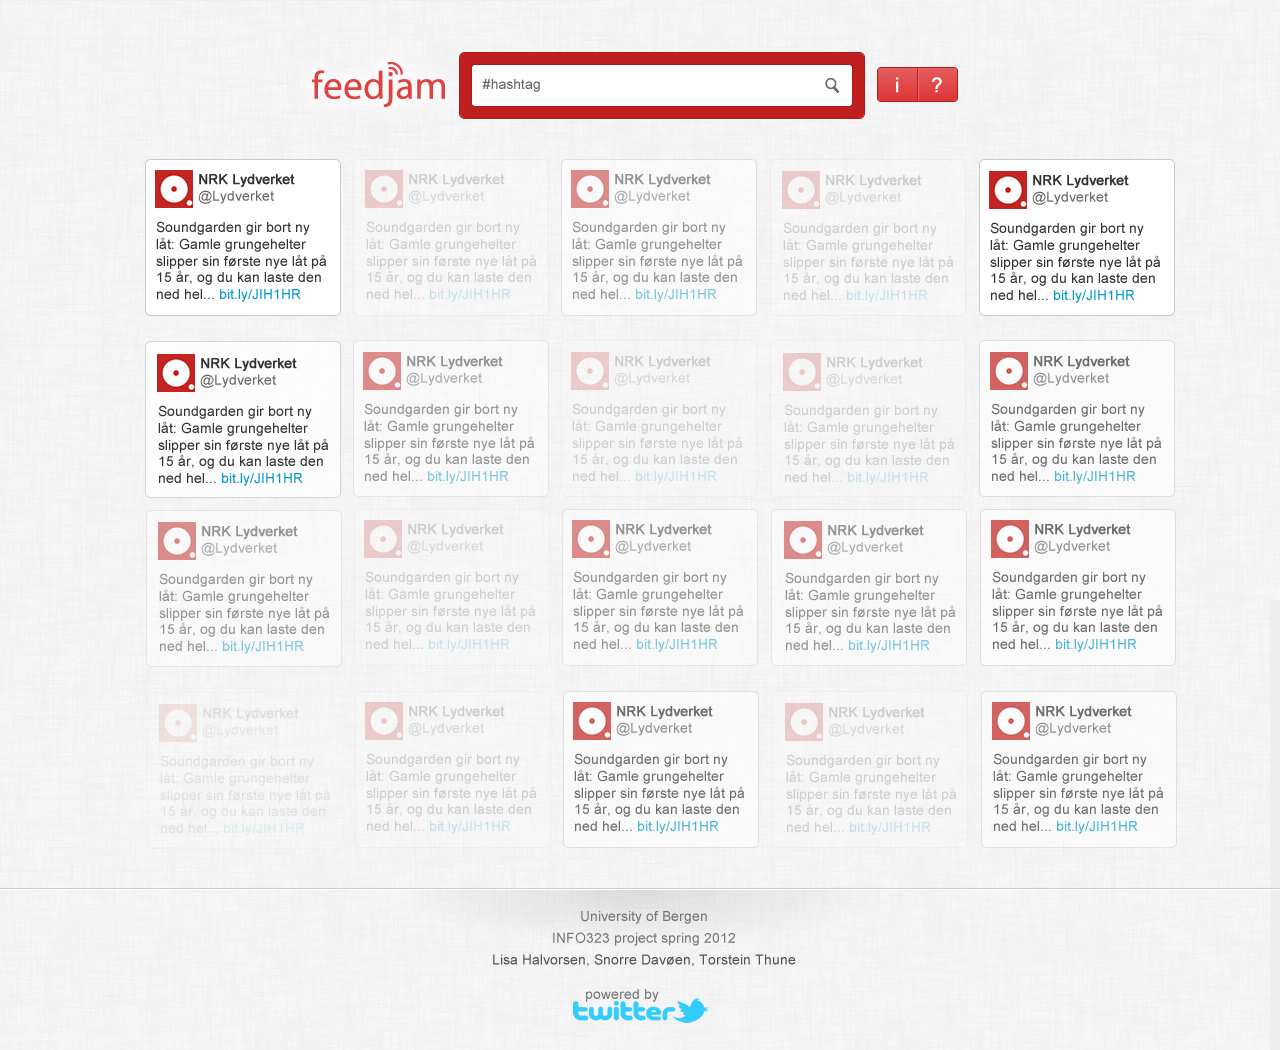
\includegraphics[width=\textwidth]{figures/layout_transparency}
        \caption{FeedJam concept using transparency}
        \label{fig:FeedJamTransparency}
    \end{minipage}
\end{figure}

Since our ranking algorithms has an output in the form of a float number (a number betweet 0.0 and 1.0) we decided that opacity, whose CSS operator can take in values in a float format, would be better since we would be able to display the nuances of our ranking algorithm to within two decimals.

\subsubsection{The final layout}
When visiting the FeedJam application homepage the users are presented with a clean layout consisting of a header containing a search form, a list of trending topics and a footer containing information about us, the creators. 

The search form consists of a standard, though large, search input field and a search button, thus providing both good visibility, since the form is very prominent, and affordance, since users are used to the concept of a search box and thus knows how to use it.

When entering a search term and clicking the search button (or when clicking a trending topic) the front page fades out, and a loading bar appears displaying information about what is being done. While the site exhibits unusual form behaviour, e.g not causing a page reload when clicking submit, this loading bar, with its connected loading messages shows the user that something has happened and that something is still happening, thus fulfilling the feedback design principle.


\subsubsection{Coding of the layout}
The frontend is coded using standard HTML5 for markup, CSS3 for styling and Javascript for front-end logic. In addition we use JSPs, which are in essence compiled template files which are used to generate the views presented to the user.

The frontend is organised in several views. Roughly we can divide these views into two categories: main views and views which are included into other views. FeedJam has one main view called home.jsp. This view is generates the markup which the user is presented with when he/she first visits the feedjam website. The home view also uses the views footer.jsp which contains the markup for the footer (bottom of page), htmlheader.jsp which contains javascript declarations and jQuery initialisation and header.jsp which contains the search form. Other views is the tweetList.jsp view and the trendingList.jsp view which are used to generate grids of tweets and a slider of trending topics. These are placed dynamically within the home.jsp view through the use of Javascript.

In order to make the site function more dynamically we use a technique called AJAX (Asynchronous Javascript and XML) coupled with JSON and HTML. AJAX is a relatively new technique for dynamically running requests and using the returned data in some way using Javascript without causing page reloads. This also makes us able to do all the API calls to Twitter through each individual user's own browser, thus making the site able to serve up to 150 searches per user per hour as opposed to a total of 150 searches for the whole web application if we were to do these requests server-side. The data is then processed server side, and a view is returned to the client, which then inserts this dynamically into the already generated view.

In order to ease the AJAX calls in addition to ensuring that the Javascript works cross-browser we use a Javascript library called jQuery. This library provides easy-to-use methods for initiating both POST and GET requests in order to providing a good interface for DOM-manipulation.


%Backend: Spring, Spring mvc, maven,  DAO, factorys, running on java servers, db more in db section,  developement
\subsection{Backend} %Serverside?
The application is developed in Spring MVC framework. FeedJam has tree controllers. The HomeController handles the trend requests for from the front page. It finds the time of the request and uses the MySQLTrendingFactory class to search the database for trends. If the trend exist in the database they are returned to the view. If trends for the current hour don't exist in the DB, a request is sent to Twitter. The response is cached and sent to the view. More on the database structure in section \ref{feedJamDatabase} \nameref{feedJamDatabase}.

AjajController handles all search requests. When the client has retrieved search results from Twitter, the Json response is posted to AjajController. Using the MySQLUserFactory, it queries the database to check if user information of the tweet owners is cached. If some users don't exist in the database, a response is sent to the view. It contains a Json array of users the client needs to retrieve information about. 
The AjajConntroller then receives a POST containing the the information on the remaining users information. New users and the Tweets are inserted to the database and a TweetSearchResult object is created. The result contains the requested Tweets with associated user information. The result is then sent as a response to the view. When the client has received the response from the server it requests the users followers and following. The list containing these users is sent to AjajController which uses MySQLUserFactory to inserts them to the database. 

The SearchController is now used as a back up. It originally handled server side requests to Twitter. %more on this? json ++




%Ranking: implementation, reference
\subsection{Ranking} %lisa
\label{ranking}
When a user enters a search term FeedJam collects response from the Twitter search API. This API has some restrictions (read more on )%using search
The consequences of this is that FeedJam only can present new tweets. Because of the limitations on the information that is possible to receive from the Twitter API the FeedJam TweetRanking function is very simple. The idea is that Tweets containing specific markup are more valuble, but if a Tweet contains to many markups it probably is a spam Tweet \citep{}.%Find spam ref
The Mentions markup is used to annotate Twitter users in at Tweet. A Tweet that mentions another user will show on the other users profile timeline.
A Tweet receives zero points i

The results are ranked by the FeedJam Rank which is a combination of User Rank (based on Page Rank) and TweetRank. The UserRank uses the information about the tweeters followers and the users the tweeter follows. The relation between user/follower/following represents the link relation between pages in PageRank. The idea is that tweeters with many followers are interesting. They get many followers because they have something interesting to tweet about. 

%caching DB 
\subsection{Database} %lisa
\label{feedJamDatabase}




TweetRank
A tweet is considered “good” if it’s read by many. 
se på retweets of antall følgere de som har retweetet har.
-hvis en tweet fra en bruker med lav userRank er retweetet av brukere med mange følgere/høy userRank blir tweetRank høy -> lav UserRank + høy TweetRank = middels FeedJamRank
-hvis en tweet er tweetet and en bruker med høy UserRank men ikke retweetet -> høy UserRank + law TweetRank = middels FeedJamRank.
- Høy userRank + Høy tweetRank = høy FeedJamRank
HashTags: 0-1 = 1, 2-3 = 2; 4++ = 0
Av de 100
TweetRank = sum(retweeters follwers rank)
log skala

